\documentclass[11pt,psfig]{article}
\usepackage{epsfig}
\usepackage{times}
\usepackage{amssymb}
\usepackage{float}
\usepackage{listings}
\usepackage{graphicx}
\usepackage{caption}
\usepackage{subcaption}

\newcount\refno\refno=1
\def\ref{\the\refno \global\advance\refno by 1}
\def\ux{\underline{x}}
\def\uw{\underline{w}}
\def\bw{\underline{w}}
\def\ut{\underline{\theta}}
\def\umu{\underline{\mu}} 
\def\bmu{\underline{\mu}} 
\def\be{p_e^*}
\newcount\eqnumber\eqnumber=1
\def\eq{\the \eqnumber \global\advance\eqnumber by 1}
\def\eqs{\eq}
\def\eqn{\eqno(\eq)}

 \pagestyle{empty}
\def\baselinestretch{1.1}
\topmargin1in \headsep0.3in
\topmargin0in \oddsidemargin0in \textwidth6.5in \textheight8.5in
\begin{document}
\setlength{\parskip}{1.2ex plus0.3ex minus 0.3ex}


\thispagestyle{empty} \pagestyle{myheadings} \markright{Homework
2: CS 217 Spring 2015}



\title{CS 217 Homework 2}
\author{Zachary DeStefano, 15247592}
\date{Due Date: May 12, 2015}

\maketitle

\vfill\eject

\newpage

\section*{Problem 1}

The following are examples of running the SIFT matching code on my own objects

\subsection*{Squirtle Example}

Figure \ref{squirtleOriginal} shows the original pictures that I took of a stuffed Pokemon named Squirtle. 

\begin{figure}
        \centering
        \begin{subfigure}[b]{0.4\textwidth}
                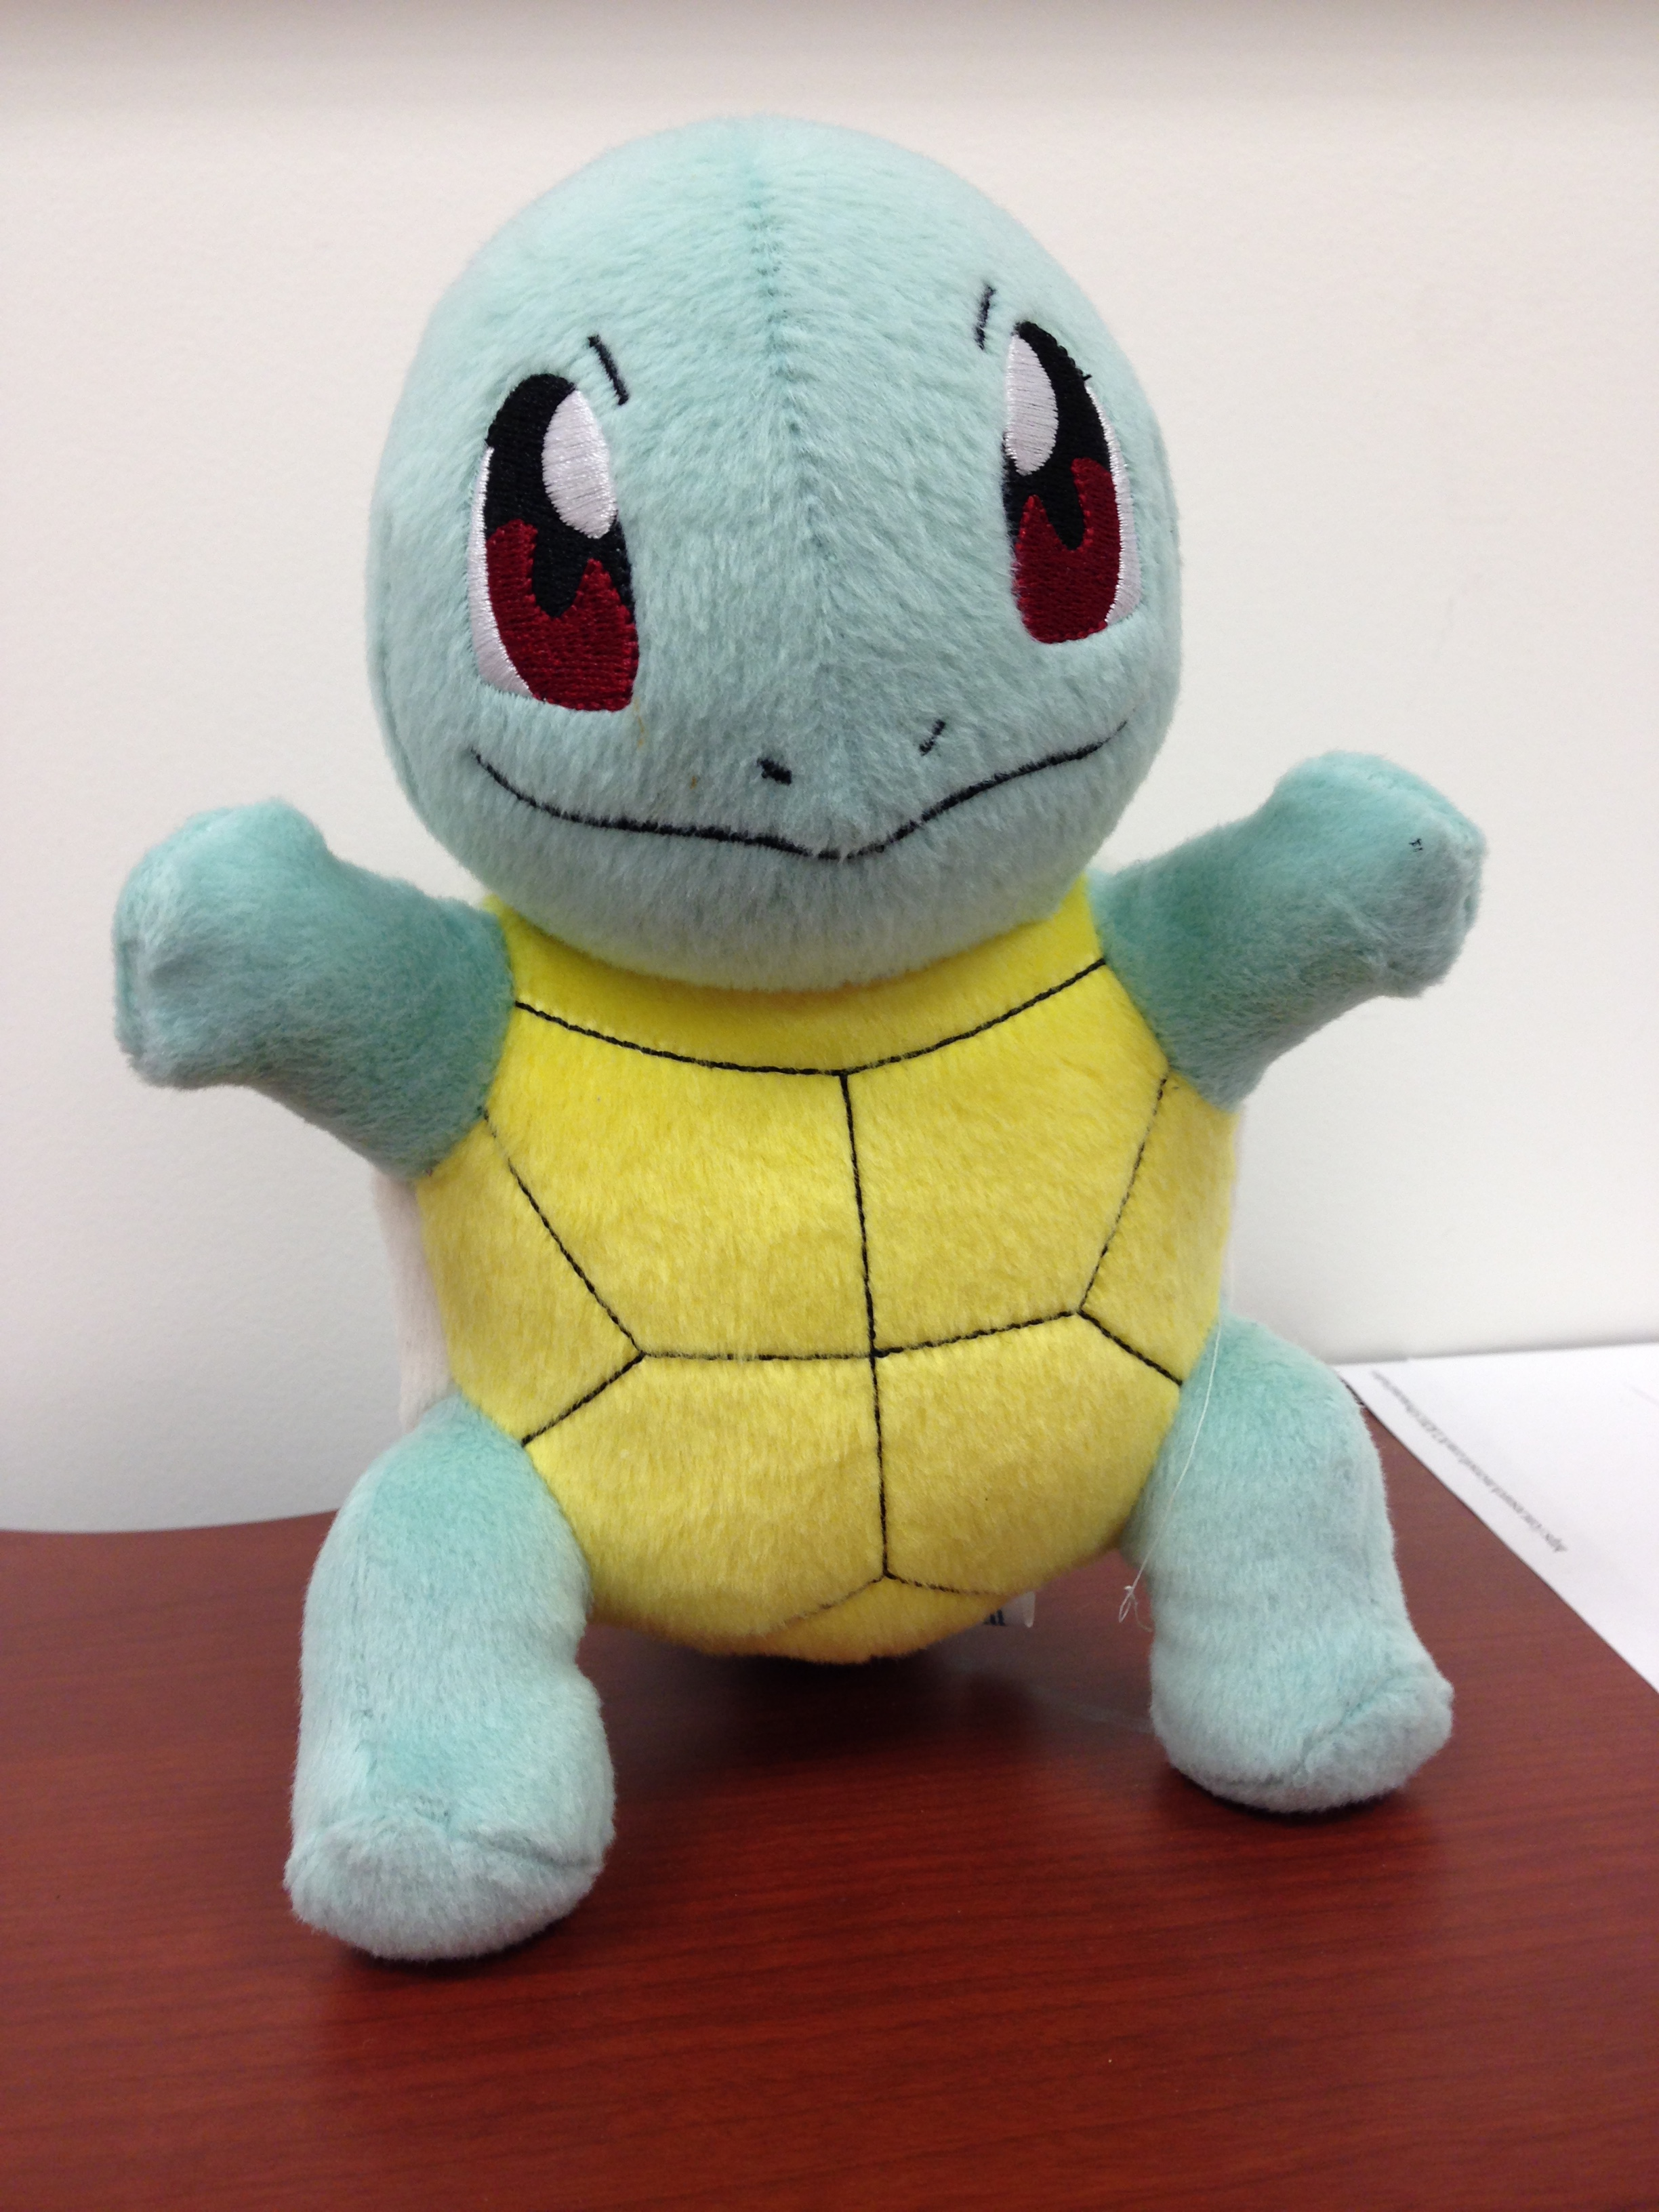
\includegraphics[width=\textwidth]{squirtle1.jpg}
		\caption{Left Image}
        \end{subfigure}
        \begin{subfigure}[b]{0.4\textwidth}
                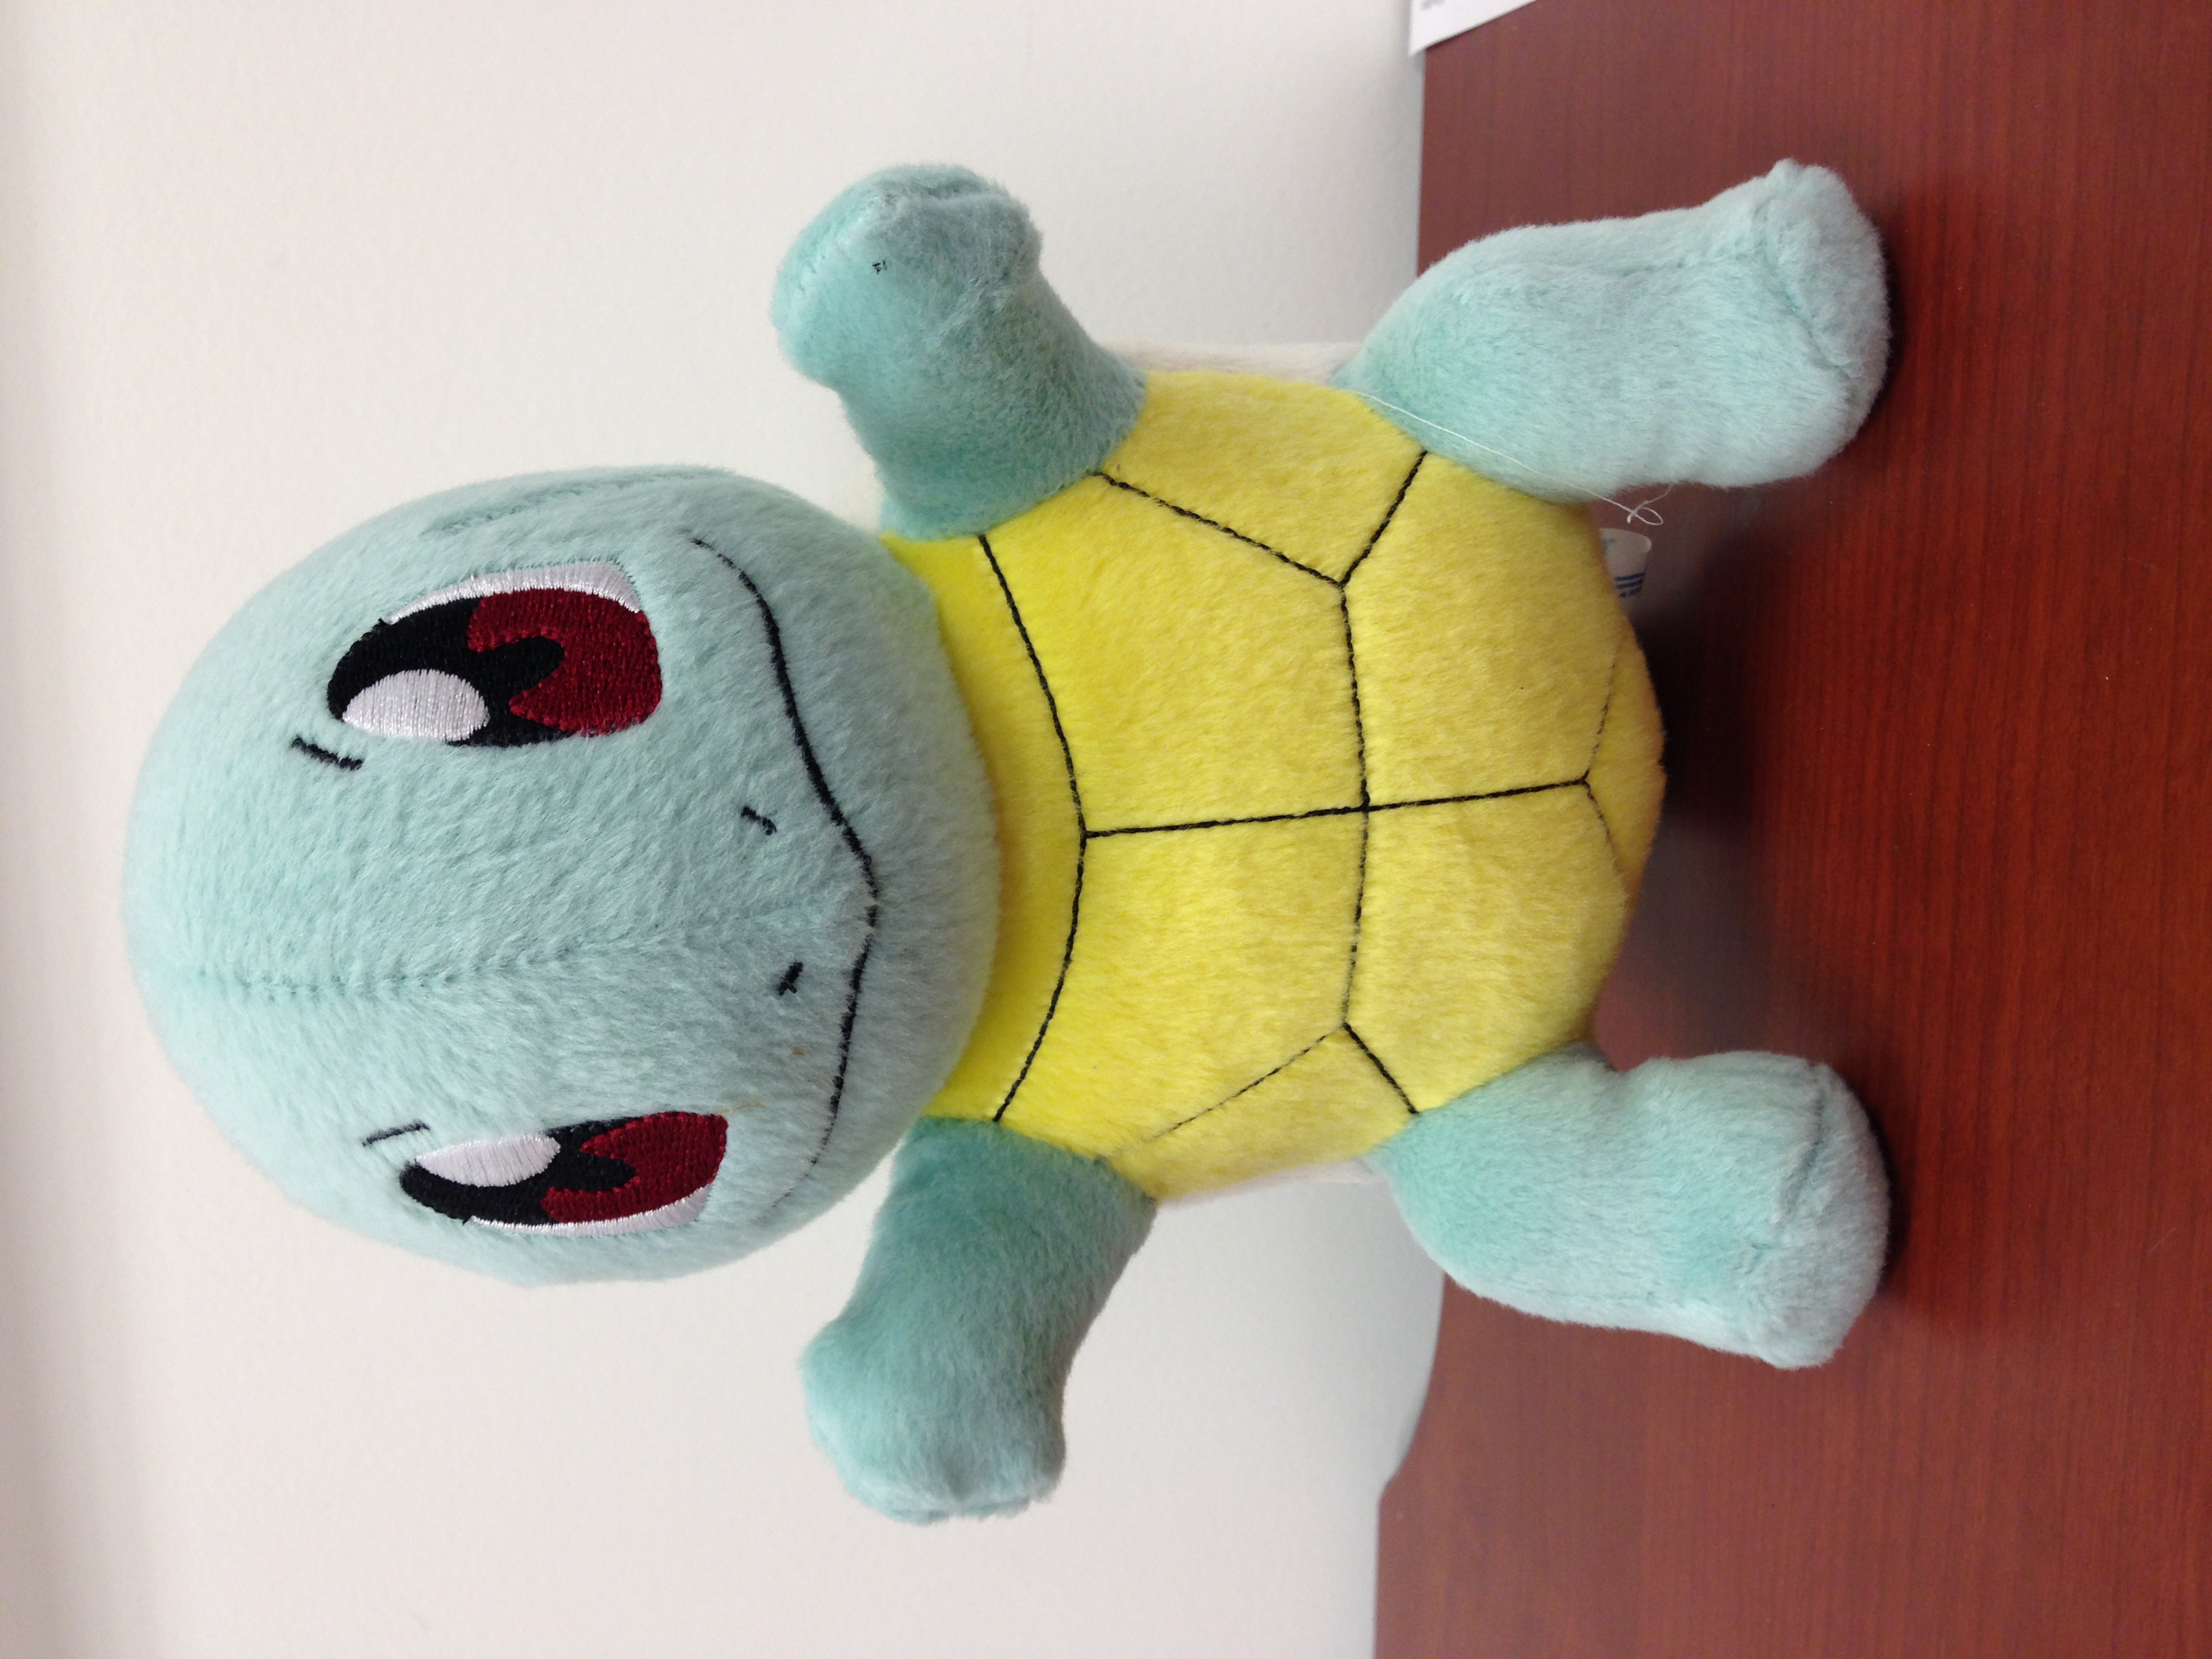
\includegraphics[width=\textwidth]{squirtle2.jpg}
                \caption{Right Image}
        \end{subfigure}
        \caption{Original Pictures of Stuffed Squirtle}
        \label{squirtleOriginal}
\end{figure}

\begin{figure}[H]
\centering
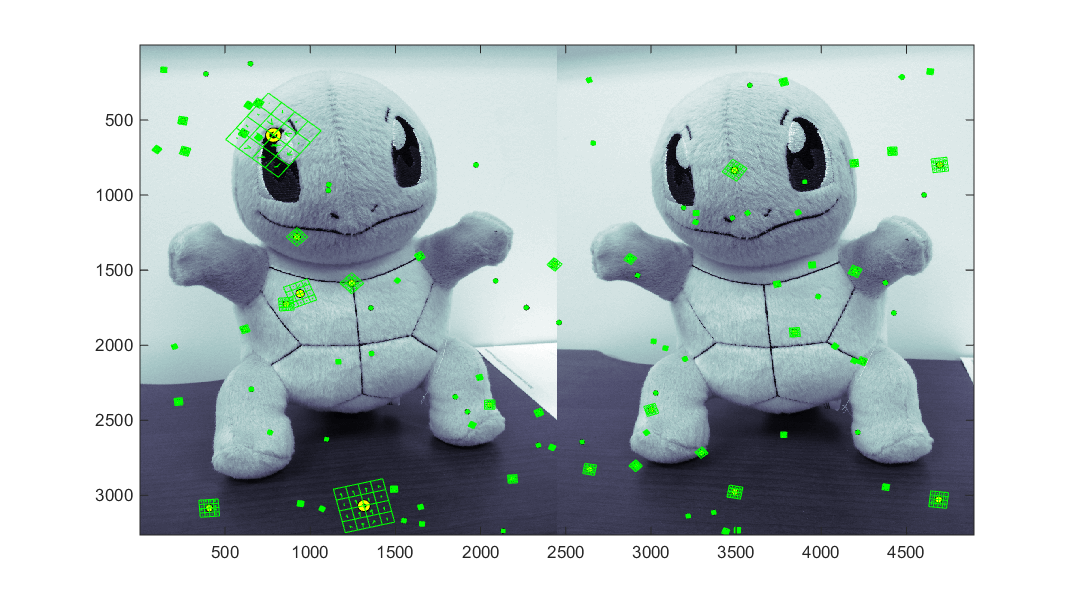
\includegraphics[height=4in]{squirtle_pointsWoMatching.png}
\caption{Squirtle Images With Points Marked}
\end{figure}

%\lstinputlisting[firstline=1, lastline=54]{triangulate.m}


\end{document}








